\documentclass[a4paper,10pt]{article}
\usepackage{amsmath}
\usepackage{graphicx}
% If you want to use Chinese, include the following package
\usepackage{CJKutf8}
\usepackage{color}

\title{CS5321 Numerical Optimization Homework 1}
\author{Due Oct 28}
\date{}
\begin{document}
\maketitle
\begin{enumerate}
 \item (30\%) For a single variable unimodal function $f \in [0, 1]$, we want to find its minimum.  We have introduced the binary search algorithm in the class.  But in each iteration, we need two function evaluations, $f(x_k)$ and $f(x_k+\epsilon)$.  Here is another type of algorithms, called ternary search. Figure \ref{fig1} illustrates the idea.  The initial triplet of $x$ values is $\{x_1, x_2, x_3\}$.   
\begin{figure}[h]
\centering
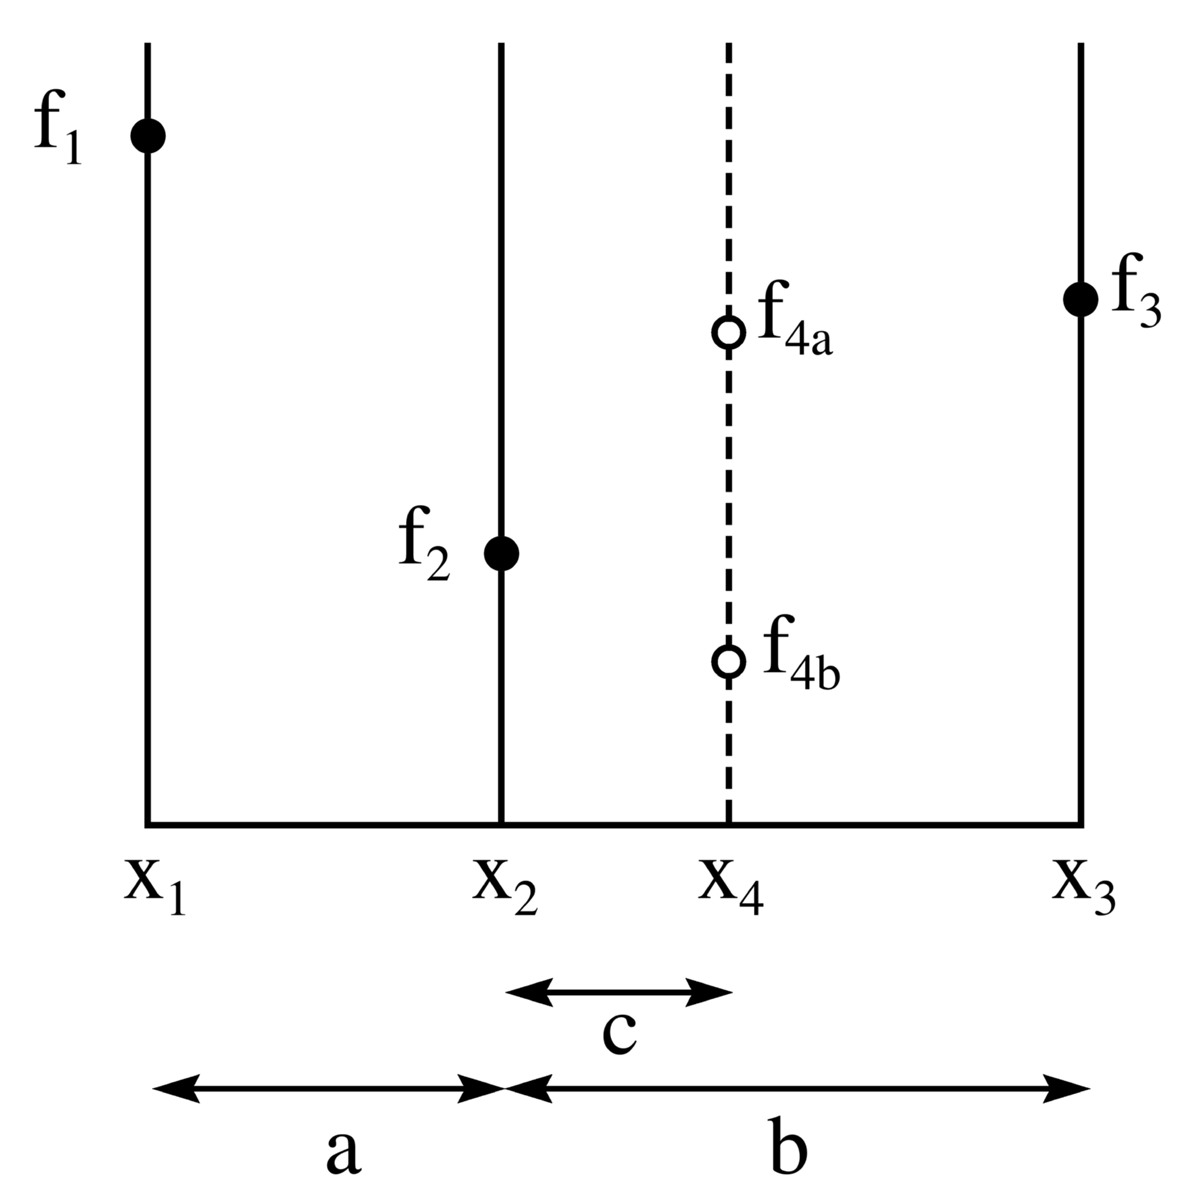
\includegraphics[scale=0.1]{GoldenSectionSearch.png}
\caption{The idea of ternary search.}
\label{fig1}
\end{figure}

{\color{blue} Answers are put here. 

    \begin{CJK*}{UTF8}{bsmi}
也可以使用中文回答
\end{CJK*}

}


\begin{enumerate}
		\item (10\%) For the search direction, show that to find the minimum point, if $f(x_4)=f_{4a}$, the triplet $\{x_1,x_2,x_4\}$ is chosen for the next iteration. If $f(x_4)=f_{4b}$, the triplet $\{x_2, x_4, x_3\}$ is chosen. (Hint: use the property of unimodal.)
    \item (10\%) For either case, we want these three points keep the same ratio, which means
    $$\frac{a}{b} = \frac{c}{a} = \frac{c}{b-c}.$$
    Show that under this condition, the ratio of $b/a=(\sqrt{5}+1)/2$, which is the golden ratio $\phi$. (So this algorithm is called the \emph{Golden-section search}).
    \item (10\%) If we let each iteration of the algorithm has two function evaluations, show the convergence rate of the Golden-section search is  $\phi^{-2}$.  (This means it is faster than the binary search algorithm under the same number of function evaluations.)  
    \end{enumerate}

{\color{blue} Answers are put here. 

    \begin{CJK*}{UTF8}{bsmi}

\end{CJK*}

}

\item (15\%) Show that Newton's method for single variables is equivalent to build a quadratic model 
$$q(x) = f(x_k) + f'(x_k)(x-x_k) + \frac{f''(x_k)}{2}(x-x_k)^2$$
at the point $x_k$ and use the minimum point of $q(x)$ as the next point.  (Hint: to show the next point $x_{k+1} = x_k -f'(x_k)/f''(x_k)$) 

{\color{blue} Answers are put here. 

    \begin{CJK*}{UTF8}{bsmi}

\end{CJK*}

}

\item (15\%) Matrix $A$ is an $n\times n$ symmetric matrix.  Show that  
all $A$'s eigenvalues are positive if and only if $A$ is positive definite. 

{\color{blue} Answers are put here. 

    \begin{CJK*}{UTF8}{bsmi}

\end{CJK*}

}

  \item (50\%) Consider a function $f(x_1,x_2) = (x_1-x_2)^3+2(x_1-1)^2$. 
    \begin{enumerate}
    \item Suppose $\vec{x}_0=(1,2)$. Compute $\vec{x_1}$ using the steepest descent step with the optimal step length.

{\color{blue} Answers are put here. 

    \begin{CJK*}{UTF8}{bsmi}

\end{CJK*}

}

    \item What is the Newton's direction of $f$ at $(x_1,x_2)=(1,2)$?  Is it a descent direction?

{\color{blue} Answers are put here. 

    \begin{CJK*}{UTF8}{bsmi}

\end{CJK*}

}

    \item Compute the LDL decomposition of the Hessian of $f$ at $(x_1,x_2)=(1,2)$. (No pivoting)


{\color{blue} Answers are put here. 

    \begin{CJK*}{UTF8}{bsmi}

\end{CJK*}

}
    \item Compute the modified Newton step using LDL modification.

{\color{blue} Answers are put here. 

    \begin{CJK*}{UTF8}{bsmi}

\end{CJK*}

}
    \item Suppose $\vec{x}_0=(1,1)$ and $\vec{x}_{1}=(1,2)$, and the $B_0=I$. Compute the quasi Newton direction $p_1$ using BFGS.

{\color{blue} Answers are put here. 

    \begin{CJK*}{UTF8}{bsmi}

\end{CJK*}

}

    \end{enumerate}


\end{enumerate}



\end{document}
